\chapter{Svolgimento stage}
\label{cap:svolgimentoStage}
In questo capitolo vengono descritte tutte le attività da me svolte durante lo \emph{stage}, divise nelle sezioni “Analisi”, “Progettazione”, “Programmazione” e “Verifica e validazione”, in modo da fornire una panoramica chiara e strutturata del lavoro svolto, evidenziando il processo seguito e le competenze acquisite in ciascuna fase.\\
Esse non sono intese come completamente sequenziali bensì, fin dalla prima fase, sono presenti tutte le attività correlate in modo da coprire l'intero periodo di \emph{stage}.\\
\section{Analisi}
In questa sezione sono presenti tutte le attività analitiche da me svolte e il suo scopo è descrivere le modalità con cui ho compreso i bisogni, i requisiti e le tecnologie del mio progetto di \emph{stage}.\\
Essendo quest'ultimo focalizzato per la maggior parte su attività legate alla ricerca e all'esplorazione tecnologica, la fase di analisi rappresenta la parte più corposa delle mie attività.\\

\subsection{Requisiti}
I requisiti del mio \emph{stage}, derivanti in parte dalle dichiarazioni aziendali presenti nel documento “Progetto Formativo” generato all'inizio del suo svolgimento, e in parte conseguenza dell'analisi dei requisiti avvenuta in corrispondenza con la presenza di specifiche necessità progettuali, sono divisi in categorie:
\begin{enumerate}
	\item[O -]requisiti obbligatori, vincolanti in quanto obiettivi primari richiesti dall'azienda.
    \item[D -]requisiti desiderabili, non strettamente necessari ma dal riconoscibile valore aggiunto.
    \item[F -]requisiti facoltativi / opzionali, rappresentanti un valore aggiunto non strettamente competitivo.\\
\end{enumerate}
Essi sono:
\begin{table}[htbp]
    \label{tab:obiettiviProgettuali}
    \renewcommand{\arraystretch}{1.5}
    \begin{tabularx}{\textwidth}{|l|X|l|}
    \hline
    \textbf{Codice} & \textbf{Descrizione}\\
    \hline \textbf{O1}    & Comprensione e mappatura delle funzionalità possibili tramite l'adozione dell'applicazione Microsoft Power Automate.\\
    \hline O1.1  & Analisi approfondita riguardo ai flussi Power Automate ed individuazione delle caratteristiche, positive e negative, della sua adozione in azienda.\\
    \hline O1.2  & Sviluppo collaborativo sui flussi Power Automate.\\
    \hline O1.3  & Produzione ed esposizione al \emph{tutor} aziendale e al \emph{team} di sviluppo di una presentazione riguardo ai risultati della mia analisi sull'adozione di Power Automate in azienda.\\
    \hline \textbf{O2}  & Comprensione ed utilizzo della tecnologia Microsoft Power Apps e relative fasi di sviluppo collaborativo.\\
    \hline O2.1  & Comprensione di Power Apps affiancando il \emph{team} di sviluppo fino al raggiungimento della comprensione dei metodi lavorativi e dei prodotti aziendali sviluppati con tale strumento.\\
    \hline O2.2  & Identificazione e definizione di un metodo adatto allo sviluppo collaborativo di applicazioni Power Apps.\\
    \hline O2.3  & Ottenimento di avanzamenti nello stato dei lavori di applicazioni aziendali realizzate con Power Apps.\\
    \hline \textbf{O3}  & Individuazione ed implementazione di un efficace sistema di versionamento per progetti realizzati utilizzando tecnologie Power Automate e Power Apps\\
    \hline \textbf{O4}  & Comprensione delle metodologie \gls{DevOps} e realizzazione della documentazione relativa alla sua applicabilità su tecnologie Power Automate e Power Apps.\\
    \hline
    \hline \textbf{D1}  & Collaborazione con gli altri stagisti universitari e individuazione di soluzioni collaborative relative ai bisogni progettuali comuni.\\
    \hline \textbf{D2}  & Realizzazione di PoC a supporto delle soluzioni individuate durante le fasi di ricerca.\\
    \hline D2.1  & Realizzazione di PoC riguardo allo sviluppo di flussi Power Automate approvativi.\\
    \hline D2.2  & Realizzazione di PoC riguardo all'integrazione tra flussi Power Automate ed elementi esterni tramite le chiamate \gls{http}.\\
    \hline D2.3  & Realizzazione di PoC riguardo al processo \gls{DevOps} di \emph{build} su progetti realizzati con tecnologie Power Automate/Power Apps.\\
    \hline D2.4  & Realizzazione di PoC riguardo all'applicazione di analisi statica del codice su progetti realizzati con tecnologie Power Automate/Power Apps.\\
    \hline D2.5  & Realizzazione di PoC riguardo al processo \gls{DevOps} di \emph{test} su progetti realizzati con tecnologie Power Automate/Power Apps.\\
    \hline \textbf{D3}  & Esecuzione di \emph{meeting} e scambio di documenti con gli altri stagisti universitari al fine di comprendere l'applicabilità delle fasi di \gls{DevOps} in ambito \gls{Sistemi} \\
    \hline
    \hline \textbf{F1}  & Esplorazione della tecnologia Angular mediante realizzazione di un progetto di \emph{test}\\
    \hline \textbf{F2}  & Integrazione di un progetto Angular con le fasi di \gls{DevOps} mediante un \emph{server} Jenkins.\\
    \hline \textbf{F3}  & Realizzazione ed esposizione di una presentazione finale, in collaborazione con gli altri stagisti, riguardo tutto il lavoro fatto durante lo \emph{stage}.\\
    \hline
    \end{tabularx}
    \caption{Tabella dei requisiti progettuali.}
\end{table}%
\subsection{Ambiente di lavoro}
Durante i primi giorni dello \emph{stage} sono stato introdotto all'ambiente di lavoro e alle tecnologie di comunicazione e collaborazione.\\
Conseguentemente ho analizzato e utilizzato il sistema di messaggistica basato su Microsoft Teams e Outlook e ho compreso la struttura di condivisione dei dati, utilizzata in azienda, basata sullo strumento Microsoft SharePoint.\\
Esso è una piattaforma \emph{software} in grado di organizzare dati sottoforma di \emph{file} e strutture tabellari chiamate “Liste”, al fine di gestire il materiale condiviso dall'azienda e dai singoli \emph{team} tramite un sistema di accessi e autorizzazioni.\\

Tramite questi strumenti ho studiato i documenti aziendali a me forniti in modo da comprendere i principali processi produttivi di Wintech.\\ 
Tali documenti comprendono i “Documenti di sviluppo sicuro” e includono:
\begin{itemize}
    \item Agile e SCRUM: descrizione delle metodologie Agile e SCRUM, spiegazione dei ruoli necessari e delle cerimonie previste. 
    \item Presentazione sviluppo sicuro: presentazione PowerPoint che descrive i processi aziendali atti a migliorare la qualità dei prodotti realizzati automatizzando fasi ripetitive e rispettando criteri di sicurezza. 
    \item Modelli di sviluppo sicuro: elenco dettagliato dei documenti di sviluppo sicuro i quali descrivono come applicare automazioni processuali (per esempio i processi di \emph{build} e \emph{deploy}) in modo sicuro e normato. 
    \item Politiche di sviluppo sicuro: strategie e normative aziendali definite al fine di garantire sicurezza e qualità nei processi e nel ciclo di vita del \emph{software}. 
    \item Piani di progetto degli altri stagisti: piani formativi degli altri due stagisti che nel mio stesso periodo hanno effettuato lo \emph{stage} universitario in Wintech. 
\end{itemize}
Relativamente a quest'ultimo punto, nei primi giorni ho approfondito il lavoro svolto dagli altri stagisti tramite appositi \emph{meeting} nei quali mi hanno descritto i risultati ottenuti fino a quel momento. Essi, avendo iniziato lo svolgimento del progetto circa una settimana prima, mi hanno esposto, mediante apposite presentazioni PowerPoint, le proprie ricerche riguardanti l'utilizzo dello strumento Git e dello studio avvenuto riguardo la possibilità di integrare tra loro gli strumenti Planner e Taiga. 

\subsection{Tecnologie oggetto di stage}
In questo sottocapitolo vengono descritti i metodi di apprendimento e le nozioni apprese durante la fase di analisi delle tecnologie su cui si basa la ricerca del mio progetto di \emph{stage}.\\\\
Dopo aver compreso le tecnologie e i principali processi aziendali, ho partecipato ad un \emph{meeting} con il \emph{tutor} aziendale al fine di discutere il mio progetto di \emph{stage}.\\
I requisiti scaturiti da tale incontro sono stati: 
\begin{itemize}
    \item Autoapprendimento dello strumento Power Automate.
    \item Realizzazione di un PoC che testasse la possibilità di realizzare un flusso approvativo Power Automate. 
    \item Testare le funzionalità disponibili con le licenze di utilizzo \emph{standard}. 
\end{itemize}

\subsubsection*{Power Automate}
Ho pertanto studiato approfonditamente tali tecnologie con l'ausilio delle numerose guide e \emph{tutorial} offerti da Microsoft. 
Essi sono direttamente accessibili dalla \emph{home} di Power Automate e Power Apps e sono divisi in moduli testuali corredati da immagini, dalla durata e argomenti specifici. 

\begin{figure}[htbp] 
    \centering 
    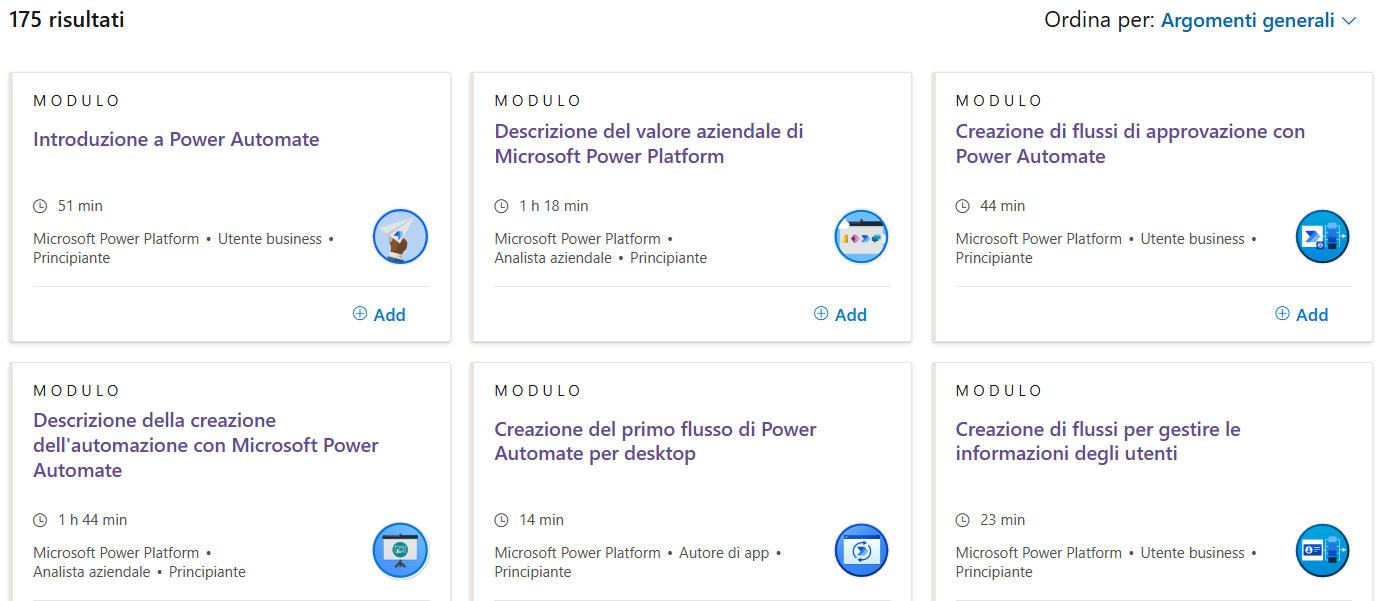
\includegraphics[width=0.8\columnwidth]{moduliPowerAutomate} 
    \caption{Moduli formativi per Power Automate.}
    \label{fig:moduliPowerAutomate}
    \vspace{1mm}
    Fonte: \url{https://learn.microsoft.com/it-it/training/browse/?products=power-automate}.
\end{figure}

\noindent Lo studio di tali moduli mi ha permesso di comprendere il funzionamento e le \emph{features} principali di Power Automate:\\
Esso è formato da una pagina \emph{web} che offre controllo sui flussi di automazione creati: è possibile modificarli e visualizzarne i dettagli, le esecuzioni e le statistiche. È possibile creare dei nuovi flussi partendo da altri progetti pubblici, o a noi condivisi, e modelli offerti da Microsoft da adattare alle proprie esigenze.\\
La modifica di un flusso non avviene mediante la scrittura di codice tramite un linguaggio di programmazione bensì tramite una composizione “a blocchi” personalizzabili collegati tra loro ciascuno avente proprietà e attributi definiti.\\
Essi sono selezionabili da una lista di blocchi relativi ciascuno a una funzionalità specifica di un servizio Microsoft.\\
Tali blocchi possono essere “Trigger” o “Azioni” ed entrambi sono necessari per la creazione e il funzionamento di un flusso.\\ 
In ogni flusso è presente uno e un solo Trigger il quale rappresenta il suo punto di partenza nonché la condizione che scaturisce la sua esecuzione.\\
Esistono tre tipologie principali di Trigger le quali determinano la tipologia stessa di ogni flusso:
\begin{itemize}
    \item Automatico: per esempio “SharePoint - Quando viene creato un elemento”. 
    \item Istantaneo: per esempio “Attiva manualmente un flusso”.
    \item Pianificato: per esempio “Ricorrenza”, il quale attiva il flusso periodicamente.\\
\end{itemize}

\noindent Ad ogni Trigger possono essere collegate, in serie o in parallelo, una moltitudine di Azioni, ciascuna responsabile di uno specifico compito, per esempio sono presenti le azioni “Inizializza variabile”, “Avvia e attendi un'approvazione”, “Teams - Crea una chat” e “Outlook - Invia un messaggio di posta elettronica”.\\
Sono inoltre presenti azioni dedicate alla gestione logica dei flussi come “Condizione" e “Do until”. La prima rappresenta la struttura di controllo rappresentata nei classici linguaggi di programmazione con “if”, responsabile della ramificazione dell'esecuzione del flusso in base a una condizione specifica.\\
La seconda rappresenta la struttura di controllo rappresentata nei classici linguaggi di programmazione con “Do while”, responsabile della ripetizione condizionata di un insieme di azioni garantendone sempre la prima esecuzione.
\begin{figure}[htbp] 
    \centering 
    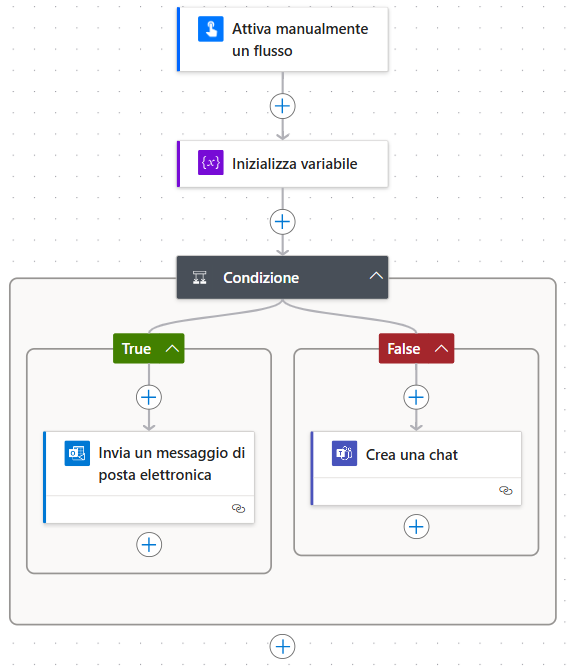
\includegraphics[width=0.5\columnwidth]{esempioFlusso} 
    \caption{Esempio di un flusso Power Automate istantaneo.}
    \label{fig:esempioFlusso}
\end{figure}
\noindent Successivamente è emersa, da parte del tutor aziendale, la necessità di integrare i flussi Power Automate con il \emph{software} gestionale WOW e gli altri prodotti aziendali al fine di poter integrare le funzionalità desiderate con libertà mantenendo coordinate le diverse parti del prodotto.\\
Sono emersi quindi due requisiti: il primo, utile per apprendere le tecnologie in oggetto, è relativo alla creazione di un flusso che automatizzi un processo approvativo.\\
Il secondo, più concreto e integrabile con i prodotti aziendali, è basato sull'applicazione, ai flussi Power Automate, di chiamate \gls{http}(Hypertext Transfer Protocol): in italiano “protocollo di trasferimento ipertestuale” è un protocollo di rete, ovvero un insieme di regole formalmente descritte che definiscono le modalità di comunicazione tra due o più apparecchiature elettroniche, usato come principale sistema per la trasmissione d'informazioni sul \emph{web}.\\
Esse permettono la comunicazione e lo scambio di dati tra flussi Power Automate e altri flussi o applicazioni: esiste infatti la possibilità di richiamare lo specifico Trigger “Alla ricezione di una richiesta HTTP” il quale genera un personale URL (Uniform Resource Locator), ovvero una sequenza di caratteri che identifica univocamente l'indirizzo di una risorsa su una rete di \emph{computer}.\\
In seguito è possibile utilizzare la corrispondente azione “Response” al fine di rispondere al chiamante con l'\emph{output} della richiesta.
\subsubsection*{Power Apps}
I flussi Power Automate portano grande vantaggio in termini di efficienza dei processi aziendali e possono aumentare il numero di funzionalità di un'applicazione.\\
Per questo motivo il loro utilizzo assume maggiore significato quando associato alla realizzazione di applicazioni Power Apps, le quali sono pensate per integrare nativamente i flussi creati.\\
Il metodo di apprendimento con cui ho analizzato e studiato Power Apps deriva non solo da attività individuali tramite i moduli didattici offerti da Microsoft nell'apposito sito \emph{web}, simili a quelli per Power Automate, ma soprattutto grazie alla collaborazione con un membro del \emph{team} di sviluppo che ho affiancato. Egli è il responsabile in azienda di tutti i loro prodotti realizzati utilizzando le tecnologie oggetto del mio \emph{stage} e assieme le abbiamo attentamente analizzate e modificate al fine di migliorarle ed applicarci le soluzioni da me individuate relativamente alle pratiche \gls{DevOps} richieste.\\
Power Apps offre la possibilità di creare nuove applicazioni e visionare le applicazioni create, o a noi condivise, con la possibilità di apportare modifiche. È inoltre possibile visualizzare informazioni e statistiche relative a tutte le applicazioni in nostro possesso.\\
Lo sviluppo di tali applicazioni non avviene esclusivamente mediante codice di programmazione bensì dall'utilizzo di componenti, \emph{standard} o \emph{custom}, che vengono manualmente posizionati sull'interfaccia, creando in questo modo una struttura gerarchica ad albero chiamata "Tree View".
\begin{figure}[htbp] 
    \centering 
    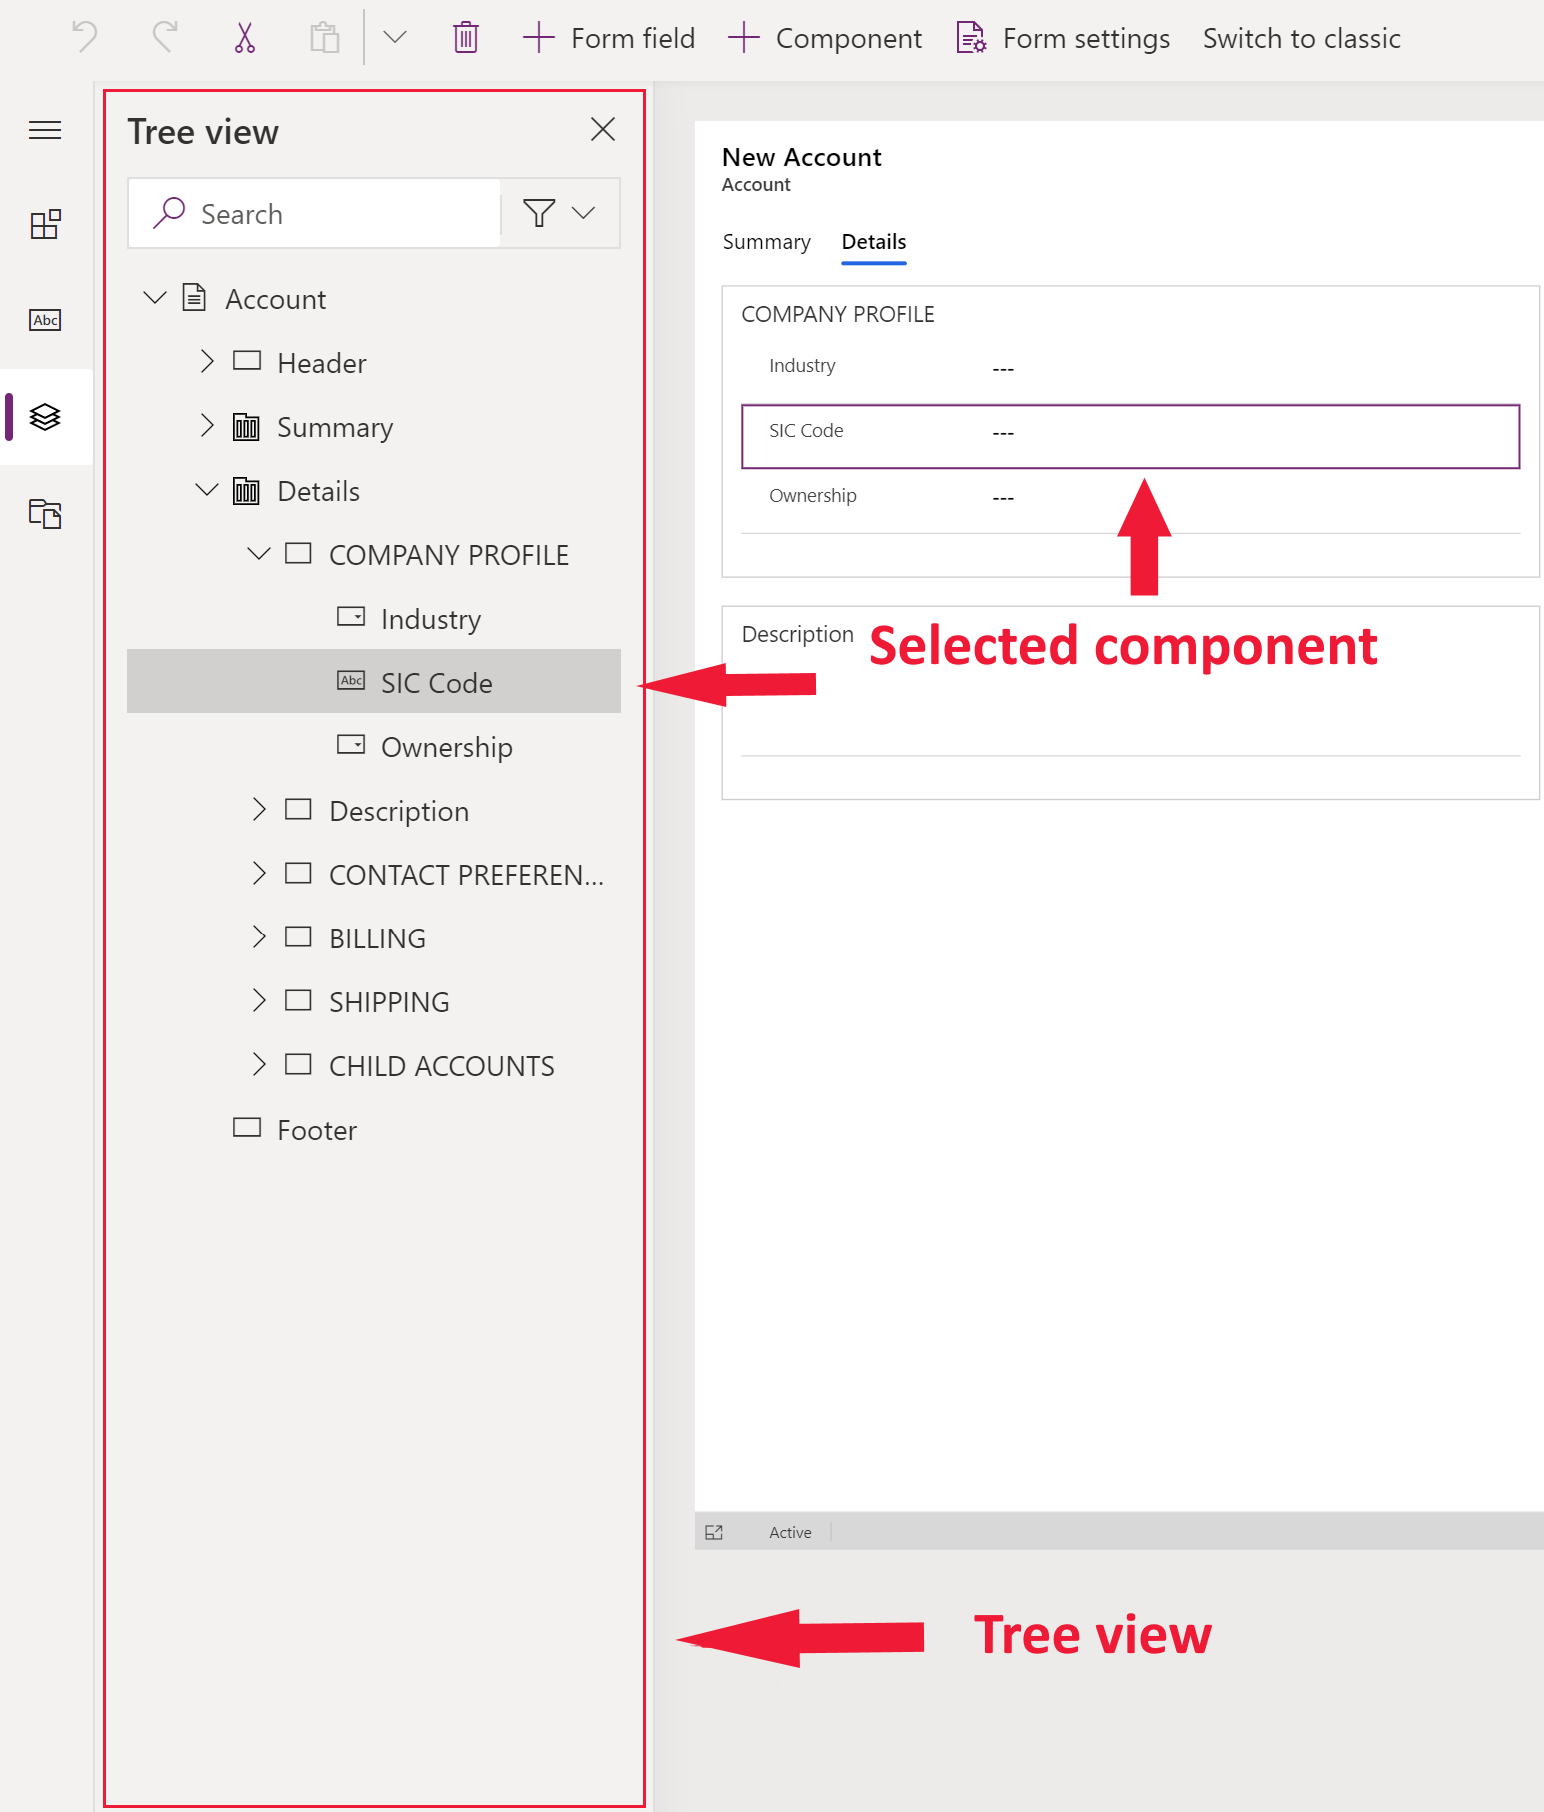
\includegraphics[width=0.6\columnwidth]{powerAppsTreeView} 
    \caption{Elemento Tree View per la gestione gerarchica dei componenti.}
    \label{fig:powerAppsTreeView}
    \vspace{1mm}
    Fonte: \url{https://learn.microsoft.com/en-us/power-apps/maker/model-driven-apps/using-tree-view-on-form}.
\end{figure}
\newpage \noindent Al fine di modificare i parametri che lo compongono, ciascun componente può essere personalizzato tramite un'apposita finestra dell'interfaccia grafica. Questo non comprende solo le peculiarità grafiche ma soprattutto il loro comportamento a seguito di azioni specifiche: per esempio è possibile creare un componente “Pulsante” e personalizzarne il campo “OnSelect” al fine di eseguire conseguentemente un flusso Power Automate e inviarne i dati di \emph{output} ad un altro componente.\\
Tali istruzioni vengono definite utilizzando Microsoft Power Fx, il quale rappresenta un linguaggio di programmazione dichiarativo, fortemente tipizzato e con uso limitato di codice, usato in Microsoft Power Platform.\\
Quest'ultima piattaforma include un insieme di strumenti e tecnologie, compresi Power Automate e Power Apps, pensati per offrire la possibilità di sviluppare prodotti \emph{software} con limitata necessità di scrivere, e conoscere, codice tramite linguaggi di programmazione.\\

\subsection{Tecnologie strumentali}
In questo sottocapitolo vengono descritti i metodi di apprendimento e le nozioni apprese durante la fase di analisi degli strumenti e delle tecnologie adottate al fine di perseguire gli obiettivi e soddisfare i requisiti di \emph{stage}.
\subsubsection*{Jenkins}
Al fine di applicare le automazioni necessarie per adottare al \emph{software} le metodologie \gls{DevOps}, come richiesto dagli obiettivi di \emph{stage}, ho individuato lo strumento Jenkins in quanto esso rispecchia perfettamente le mie necessità ed è inoltre già conosciuto e applicato dal resto del \emph{team} di sviluppo rappresentando quindi una tecnologia consolidata che non necessita di ulteriore formazione all'interno dell'azienda.\\
Ho appreso le conoscenze necessarie per studiare e utilizzare tale strumento in totale autonomia mediante la consultazione delle guide e del numeroso materiale presente \emph{online} comprese le pagine \emph{web} ufficiali di Jenkins con gli annessi video \emph{tutorial}.\\
Esso è uno strumento scritto in linguaggio di programmazione Java che viene eseguito all'interno di un \emph{web server} e offre la possibilità di creare, gestire, eseguire e monitorare dei progetti Jenkins chiamati “Job”, potendone visionare e registrare i \emph{report} di \emph{output}.\\
Essi sono unità di lavoro configurabili che rappresentano un'attività o un progetto specifico che Jenkins esegue. Possono essere di diverso tipo ma tutti sono basati sull'esecuzione di uno \emph{script} o una \emph{pipeline} di automazione.\\
Una \emph{pipeline} Jenkins è una sequenza di fasi chiamate “Stage”, eseguite in serie o in parallelo, responsabili di specifiche operazioni definite dall'utente, per esempio \emph{build}, \emph{test}, \emph{deploy}. Esse possono essere definite tramite il linguaggio di programmazione Groovy oppure tramite l'interfaccia grafica di Jenkins.\\
Questo strumento permette dunque di fornire servizi di integrazione continua ed è indicato per l'applicazione di alcune fasi di \gls{DevOps} come Build e Test, il caricamento automatico dei file sul \emph{repository} di versionamento desiderato e l'autenticazione automatica ai servizi Microsoft tramite comandi Power Platform CLI.\\
Quest'ultima è un'interfaccia a riga di comando che offre la possibiltà di eseguire un insieme di comandi specifici atti all'autenticazione e alla gestione degli ambienti e delle Microsoft Solutions.\\
\begin{figure}[htbp] 
    \centering 
    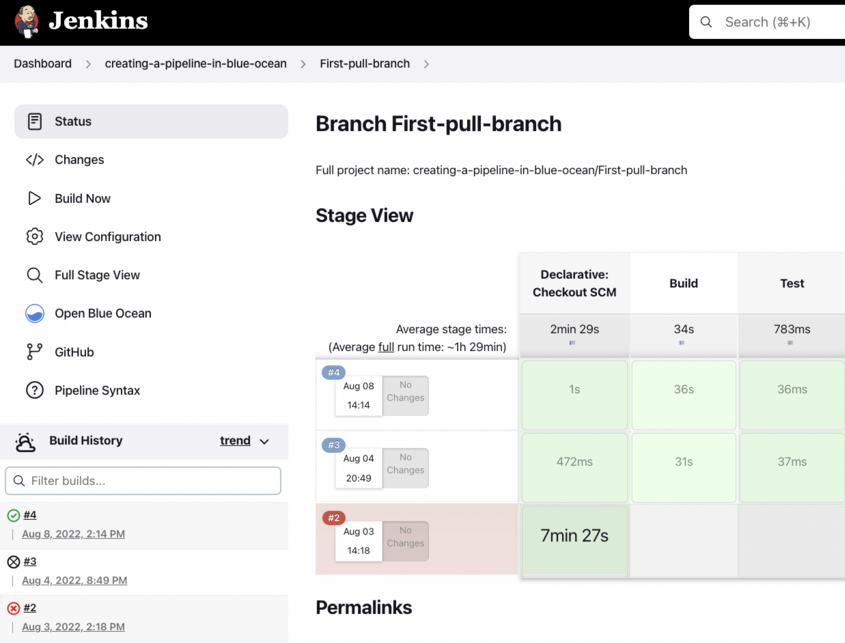
\includegraphics[width=0.9\columnwidth]{esempioJenkins} 
    \caption{Esempio interfaccia di Jenkins.}
    \label{fig:esempioJenkins}
    \vspace{1mm}
    Fonte: \url{https://commons.wikimedia.org/wiki/File:Updated-jenkins-view.png}.
\end{figure}

\subsection{Microsoft Solutions}
Un'ulteriore oggetto di analisi e studio è stato l'utilizzo e la comprensione delle Microsoft Solutions. Esse fanno parte della \emph{suite} Microsoft Power Platform e sono degli strumenti che servono a contenere tutti i flussi Power Automate e applicazioni Power Apps corrispondenti a uno stesso progetto, in modo da poterli sviluppare e distribuire in maniera organizzata e centralizzata.\\
Esistono due tipi di Soluzioni: 
\begin{itemize}
    \item Gestite: destinate prevalentemente per gli ambienti di produzione e \emph{test}, non permettono la modifica degli elementi al suo interno. Per generare una Soluzione gestita è necessario esportare una soluzione non gestita.
    \item Non gestite: destinate prevalentemente per gli ambienti di sviluppo, permettono la modifica degli elementi al suo interno e la sua esportazione.
\end{itemize}
A differenza delle tecnologie precedentemente descritte, le Micorsoft Solution non erano materia già affrontata in azienda, per cui il loro apprendimento è avvenuto in maniera totalmente autonoma mediante la documentazione presente nei siti \emph{web} Microsoft dedicati.\\
Le Soluzioni preservano i loro dati, e quelli degli elementi in esse contenuti, nel sistema di archiviazione Microsoft Dataverse che funge da \emph{database} centralizzato per applicazioni sviluppate con la Power Platform.\\
Tale adozione permette di usufruire di funzionalità altrimenti assenti. Le conseguenze del loro utilizzo e le motivazioni che mi hanno portato ad utilizzare questa tecnologia sono materia di discussione presente nel capitolo 3.2 Progettazione.\\

\subsection{DevOps}

\subsubsection*{Plan}

\subsubsection*{Code}

\subsubsection*{Build}

\subsubsection*{Test}

\subsubsection*{Release}

\subsubsection*{Deploy}

\subsubsection*{Operate}

\subsubsection*{Monitor}

\subsection{Applicazioni aziendali}

\subsection{Angular}

\section{Progettazione}
In questa sezione sono presenti tutte le attività progettuali da me svolte e il suo scopo è descrivere le modalità con cui ho individuato le soluzioni ai bisogni progettuali in modo da soddisfarne i requisiti.
\subsubsection*{Microsoft Solutions}

\section{Programmazione}
In questa sezione sono presenti tutte le attività da me svolte al fine di sviluppare e implementare le soluzioni individuate in fase di progettazione.

\section{Verifica e Validazione}
In questa sezione sono presenti tutte le attività da me svolte al fine di verificare il corretto funzionamento delle soluzioni sviluppate e il loro soddisfacimento dei requisiti progettuali.

\section{Risultati raggiunti}
\subsection{Qualitativamente}
%

\subsection{Quantitativamente}
%
